\documentclass[oneside,12pt,a4paper,smallheadings,DIV11]{scrbook}
\usepackage{pyblio,graphicx,xr,mdwlist,hyperref,titlesec,array,supertabular}
\usepackage[pdftex,outerbars]{changebar}
%\includeonly{td-c00}
% add font styles  like: ,galliard,gillsans, if you like
\hyphenation{data-base}
%\rcsInfo $Id$
\externaldocument[UG.]{UG}
\externaldocument[RM.]{td-td9}
\newcommand{\UG}{\textit{Pybliographer User's Guide}}
\newcommand{\RM}{\textit{Pybliographer Reference Manual}}
\begin{document}

\title{Pybliographer Development Guide}
\author{Fr�d�ric Gobry and Peter Schulte-Stracke}
\maketitle{}
\pagestyle{headings}
\bibliographystyle{plain}
% \begin{abstract}
%   This document introduces the next development steps for
%   \textbf{Pybliographer}. Here you find  a task list as well as more
%   detailed dicussions of related issues and problems.
% \end{abstract}
\tableofcontents
\newpage
\listoftables
\listoffigures
%\reversemarginpar
%\cleardoublepage
  \setcounter{secnumdepth}{-1}
  \section{To Do List}
\label{sec:todo}



\todoprio{For the next release}

\subsection{The Graphical User Interface}
\label{todo:next:gui}


  \begin{itemize}
  \item \Active Refactoring the \filenm{Gnome/Index.py} code. \assign{ptr}
    \begin{itemize}
    \item Documenting the new \textsc{api}.
    \item Providing for multiple index views; switching them.
    \item \Think Better data structures for widget interface -- but see
      also future gtktreeview \& associates.
    
    \end{itemize}
  \item \Done Incremental updates. \assign{ptr}

  \item \Done Combined author/title field in Index \assign{ptr}
    \begin{itemize}
    \item A better column title is needed.
    \item The formatting should be adaptable.
    \item The index must be sorted.
    \end{itemize}
  \item \Done Mark entries
    \begin{itemize}
    \item Make subsets (lists or sequences) out of marked entreis;
      associate them with a name \dots
    \end{itemize}
 
  \end{itemize}


\subsection{Miscellaneous}
\label{sec:next:misc}

\begin{itemize}
\item A progressbar (rather simple)
\item \Think A check for duplicates. (But this may need a lot of work
  and better fit into a revamped \textit{Import} module.)
\end{itemize}




\subsection{Bugfixes}
\label{sec:next:fix}

\begin{itemize}
\item Stable Working Directory for open.
\end{itemize}
\todoprio{For Release 2.0}

\subsection*{The Graphical User Interface}
\label{todo:r20:gui}

\begin{itemize}
\item Moving to \textsf{GTK 2}.

\end{itemize}


\subsection{Generalities}
\label{todo:r20:genera}

\begin{itemize}
\item Moving to \textsf{Unicode}.
\item Elementary database substructure.
\end{itemize}


%%% Local Variables: 
%%% mode: latex
%%% TeX-master: "td-td1"
%%% End: 

\addchap{Preface}
\label{cha:preface}

This document serves as the base for development of the \Pyb\
application.This document is intended to give the \Pyb\ developers both an
introduction to the application area and an reference view of the
application as vision, guidance, and motivation.  Accordingly, it is
divided into three parts:

\begin{description*}
\item [Part 1, Overview] introduces the subject area, and lists major
  sources of reference information. Then it treats design goals,
  requested and desired features and functions; it gives an overview
  of the use cases that are to be considered and an overview of teh
  architecture, and the further development.
\item [Part 2, Design Considerations] discusses major areas and
  problems of \Pyb\'s  design  in order to give the development a
  better foundation. 
\item [Part 3, Component Spacifications] contains the specifications
  for all subsystems and packages.
\end{description*}


\section{Where to Find More Information}
\label{sec:prefmore}

 Further information can be found in:
\begin{itemize*}
\item \UG, which contains explanations of the user interactions, data
  elements, and the application programming interface, and
\item \RM, which contains all
  diagrammatic and textual information grouped according to type.
\end{itemize*}

\noindent

\begin{dnote}[Comments:]
\item Comments and corrections are always welcome.
  Please address your message to:
  \url{pybliographer-general@lists.sourceforge.net}.
\end{dnote}


\subsection{Internet Sources}
\label{sec:prefinet}
The following resources are available through the Internet:

\begin{itemize}
\item \textbf{\Pyb\ home page}

  You can vivit the \Pyb\ home page on the World Wode Web using this
  address:
\cbstart
  \url{http://www.gnome.org/pybliographer}.
\cbend

\item \textbf{\Pyb\ discussion list}

  You can also participate in the discussion on the \Pyb\ general
  mailing list operated through Source Forge. See the following
  information page:\\
  \url{http://lists.sourceforge.net/mailman/listinfo/pybliographer-general}

  To subscribe send a message to:

  \url{pybliographer-general-request@lists.sourceforge.ne} with a
  subject line set to \texttt{Subject: subscribe}.

  To post a question or response on the \Pyb\ general
  mailing list, send it to:

  \url{pybliographer-general@lists.sourceforge.net}

  Include an appropiate \texttt{Subject:} line.

  See the list's archive at the following URL:\\
  \url
{http://sourceforge.net/mailarchive/forum.php?forum=pybliographer-general}.  

\item \textbf{Download area}

  You can get source code and additional information through
  \textbf{anonymous ftp} from various places. Please refer to the
  information here: 
\url {http://canvas.gnome.org:65348/pybliographer/download.html}. 

  
  \textbf{Note:} \Pyb\ is included in all major Linux distributions.
  In most cases, you will prefer to use the specially prepared package
  that your distribution offers. See \UG \ref{UG.sec:rginstall} on
  information how to obtain and install \Pyb\ using the facilities of
  your distribution.


\item \textbf{CVS access}

  You can access the current stable and unstable code on \textbf{CVS}
  at \url{cvs.gnome.org/cvs/gnome/pybliographer}.

  For information on joining \Pyb\ development address yourself to the
  mailing list.
 
  
\end{itemize}


%%% Local Variables: 
%%% mode: latex
%%% TeX-master: "DG"
%%% End: 


\part{Overview}

\chapter{Introduction}
\label{cha:intro}


\setcounter{secnumdepth}{3}
%\cleardoublepage

Pybliographer provides Reference manager services to create, load,
modify, list, read, transport, and copy descriptions of bibliographic
resources like books, articles, and electronic documents, including
derivative and private information.  In addition it helps in accessing
external databases and document repositories. 

Today, scholars and writers need efficient, consistent, and less
complex ways to work with bibliographic resources and to maintain
their existing inventory of references.  The trend in bibliography is
to integrate and share data, and to develop applications that
transcend traditional boundaries.

In the past, reference managers had only limited ability to adapt to
the plenitude of working environments and to interact with other
applications.  This has often constrained those with special needs to
work with inadequate programs, and burdened them with work-arounds and
makeshift arrangements. Bibliographic software has on the whole tended
to be idiosyncratic and limited in its outlook, or to be expensive,
complicated and nevertheless constrained to a small subset of the
requirements, as it is, e.g., the case with \textsf{MARC}-based
library software (from the point of an individual writer\slash
scholar, at least).

\Pyb\ establishes a common base for many tasks. It combines essential
services, such as database access, formatting and searching records,
with a common vocabulary and structure.  In making use of 
established practice and standards it avoids many of the problems that
other programs have when it comes to extending and inter-operating.
All of these services are available through a set of interfaces that
are easy to adapt and a fertile foundation for extensions.


Many restrictions inherent in the BibTeX database format used by
earlier versions of this program (and many competing programs) are
removed or relaxed in this version. 

This version continues to support \BibTeX\ databases to assist you in
converting to the new database structure. Subsequent releases,
however, might not support these features, so we strongly recommend
conversion to the exclusive use of the new database structure.

Support for using \BibTeX\ as an import and export format, however, is
planned for the foreseeable future.


\section{The Evolution of Bibliographical Software}
\label{sec:introevo}




As a bibliographic database manager, \textit{Pybliographer} places
itself at the intersection of various expectations, traditions, and
requirements, each of which developed originally independent, and
often in ignorance of the other, and which are still shaping the field
according to their own peculiarities, although they are getting into
closer contact recently. For orientation, it may be useful to give a
short view of some of these ancestral developments. They embody still
important principles, and may serve as benchmarks for our endeavour.
 

\subsection{Reference Managers}
\label{sec:introdocrm}

Very early the scholarly and technical document preparation has been
supported with programs to augment document sources with correctly
formatted references, of which \textit{BibTeX} may be regarded as
prime example.  Those early applications are slanted towards the
production of reference lists, almost at the exclusion of other uses,
their storage formats are implicitly defined and easy to extend, and
the building and maintaining of its data base is left to other means.

In spite of (or perhaps because of) these deficiencies these have been
very successful programs. Their restrictions, that follow a well
proved tradition after all, were intended and adequate at the time of
their creation. They have been addressed by the next class of
applications which developed, characteristically, in the highly
competitive marketplace of the \textit{personal computer}.

With the advent of the Personal Computer a new class of users came to
the fore. While the majority of the scientific\slash technical writers
(who have little choice, anyway) stayed with their \TeX\ applications,
the new users were mostly attracted to the perceived simplicity of the
word processors, and eschewed the command line and simple editors of
Unix.  Almost by necessity, the new applications stressed those
aspects of the job that the older tradition neglected. Word processor
users didn't care for the typographical refinements of \TeX, nor the
frugality and intellectual self restriction of the command line.  They
wanted simplicity and ease of use, \dots\ and over the time, they
succeeded.  The graphical user interface comes no longer as an
afterthought, it is at the centre of the development effort (often to
the detriment of the application proper).

The features of \textit{Biblioscape}, a commercial product are given
in appendix \ref{sec:biblioscapefeat}.  For us it is important to
stress \cbstart the \textit{database} aspects and \cbend pay attention
to the \textit{organising} of the references, by providing suitable
instruments, e.g., the \textit{virtual folders} of Biblioscape.


\subsection{Library Catalogues}
\label{sec:introlibs}
\cbstart

In the beginning library catalogues were nothing but simple
\textit{inventories} and they and their counterparts in archives serve
this purpose to this day.  After they became accessible to the public,
though, a number of problems arose that are still important, as are
some of the solutions.  Required by the inter-library loan services
and other fields of cooperation, \textit{cataloguing rules} were
developed, culminating in the ISBD, which set a widely accepted
standard.  
%The rules and the services never ceased to influence each other; 
The actual rules have always aimed at a compromise between precision
and cost.

\cbend



% {The legacy of the card catalogue --
%   \textsf{MARC}\protect\footnote{Although \textsf{MARC} stands for Machine
%   Readable Cataloguing, it is used here loosely but legitimately and
%   stands for the whole of classical librarian's cataloguing, of which
%   the actual MARC standard has been, in a way the epitome and
%   culmination of centuries of work. Of course, it has begun to change \dots }}
% \label{sec:the-legacy-card}

% Originally inventories for the use of the librarians only, since about
% one century, the library catalogues have become accessible to the
% public and henceforth set the standard of bibliographical description.

% At about the same time began the development of rules for the
% bibliographical description,\footnote{The \textit{Preu�ische
%     Instruktionen} and the \textit{ALA Rules} were among the first.
%   Their successors are the \textit{RAK} and the AACR2, both are in
%   turn influenced (the RAK more so) by the international
%   standardisation efforts of the \textit{ISBD}.} to enable the sharing
% of catalogue entries between libraries\footnote{Either by one library
%   providing the catalogue cards f or the majority of the libraries (in
%   the US), or by building union catalogues for the purpose of sharing
%   the holdings, too (the inter-library lending service in Germany).}
% and to enable a catalogue to be build and used \textit{compatibly}
% without annoyance by many people (which is a form of sharing, too).

% oscillating between the ideal of capturing the whole title
% page (of course, only the title page\footnote{see Robert Musil's
%   \textit{Mann ohne Eigenschaften} and the talk between General Stumm
%   von Borgwehr and the director of the Royal Library \dots}) and the
% need of coping (manually) with all this. 

Over time, the descriptions tended to grow in size. There are several
reasons for this: (i) the more items exist, the more difficult it is
to distinguish between them, the more details are thus needed, (ii) if
one tries to spread the cost over more parties, one has to accept
information that individually one might not find worthwhile, and
finally, (iii) the need for better pre-selection entails even more
information, as, e.g., abstracts, to be given.\footnote {In the
  classical catalogues one could afford to be concise, as one could
  always go and fetch the copy for actual inspection.} 

% \begin{enumerate*}
% \item the more titles exist, the more it becomes difficult to
%   distinguish between similar ones,
% \item more information is made centrally available, mostly to share the
%   cost of providing it. Such was the case in Germany, where subject
%   headings appeared in the national bibliographical database, thus
%   moving something which has traditionally been the responsibility of
%   the individual institution onwards to the \textit{Deutsche
%     Bibliothek}. To do so, additional categories needed to be defined,
%   rules set up, an authority file maintained, as it was done earlier
%   for the nucleus of the bibliographical description.
% \end{enumerate*}

It should be noted, that traditionally only books have been
catalogued, together with other physical objects, that might land in a
library (\textsf{MARC} being quite comprehensive in its scope of
materials allowed). That reflects the point of view of the librarian,
who is the custodian of these said objects, buys, lends, ranges them.
The contents are not his business.  In that his view differs from the
usual patron's view, as exemplified by the Bib\TeX\ and reference
manager software (see \ref{sec:introdocrm}).  This orientation is
slowly changing under the influence of Internet resources and
integration with patron's software (section
\ref{sec:internet-access}).\footnote{\textsf{MARC} intended, indeed,
  to support so called \textit{analytical} cataloguing as well, if
  only as a secondary task. Even the description of archival resources
  is not, or so one thought, out of its scope. This reflects the facts
  that American libraries hold archival collections to a far greater
  degree than European ones, and that these are far simpler than the
  classical European archival fonds; but remarkably this proved to be
  a failure -- a separate standard (EAD) evolved, this time based on
  XML. Perhaps the reason was the absence of any form of hierarchy in
  \textsf{MARC} databases.}

Perhaps the most important heritage from this development is the idea
of \textit{entry points}: try to establish for everything that you
catalogue well-defined and precise enough attributes and make the
database search-able for them. 

For a card catalogue this implies defining not only under which
\textit{form} an author is filed, but in addition under which author a
book is filed (if there is a choice).  The first class of
normalisations is done via \textit{authority files} the importance of
which, under the conditions of on-line catalogues, has only increased,
because it is more difficult to find entries which differ slightly
\cite{Hal98} while the so called question of the main entry has no
longer the importance it used to have.
 


\subsection{Records Management}
\label{sec:intrormapp}

Of course, the management of current administrative records (records
and document management applications) is out of the scope of
bibliographical software, mostly.  But to a degree, it would be
beneficial to be able to handle one's own documents with more ease and
consistency by adding a records management feature to the reference
manager.
 
If, as it is the case in particular in the United States, archival
resources are integrated into library systems, the idea is not far to
use the same software and the same set of rules for both kinds of
material.  The use of \textsf{MARC} for archival resources failed,
however, not because of any impossibility, but because of the cultural
inability of using the in this case inevitable multi-level description
technique.  In Germany, archivists use database systems for data
entry, in America, word processors -- neither choice is fully
adequate.

Extending the database schema to enable the description of
\textit{administrative records, personal papers,} and
\textit{manuscripts}, and collections thereof, should be taken into
consideration.


\subsection{Internet Database \& Document Access}
\label{sec:internet-access}

Although the Internet precedes the personal computer by some
years,
% \footnote{Of course, it all depends.  Arguably the first
%   personal computer was the \textsf{Alto} at \textit{Xerox Parc} from
%   the early 1970, while the switch to the \textit{IP/TCP} protocol
%   family did not occur but a couple of years later.}  
the impact of the Internet was but slowly felt. We can at this time
distinguish the following issues:
\begin{description*}
\item[Database access] in particular with the intent of adding the
  results at least partially to one's database.
\item[Document access] in particular where the document's \textsf{URL}
  forms part of the bibliographical description.
\item[Electronic documents] continue to challenge the librarian's
  profession. Ephemeral, they were often felt not to warrant the
  expense of traditional cataloguing (out of which considerations the
  \textit{Dublin Core} standard evolved), hierarchical, they stretched
  the card-bound structure of \textsf{MARC} to the limits, ever
  changing, they challenged the concepts of bibliographical unit, of
  work, and edition (see chapter \ref{cha:bibdata}).

  \cbstart It is still not clear how great the impact of electronic
  documents and collections will be.  Recent developments include the
  Library of Congress' \textsf{MODS} projects, following the lead of
  the \textsf{Dublin Core} so-called \textit{Metadata} standard. The
  idea is often to replace traditional cataloguing with less expensive
  alternatives, in the first place by placing information in the
  documents (in a deplorable concession to liguistic vanity) called
  \textit{meta data}, from where it can then be \textit{harvested}
  automatically.  Unfortunately this is not easily accomplished and
  perhaps even paradixical.
  \cbend
\end{description*}



\subsection{Integration with Document Preparation}
\label{sec:introinteg}

\begin{dnote}
\item Usability issues and the changed workflow  
\end{dnote}

\subsection{Summary of current trends}
\label{sec:introtrend}

\begin{dnote}
  \item Where are the current projects heading?
  \item What is felt to be the most pressing development today?
\end{dnote}


\section{Reference Documents}
\label{sec:introrefdoc}

The following gives a list of articles and other reference sources
that are helpful in understanding the issues.

\begin{dnote}
\item A more comprehensive list could perhaps be drawn up, in another
  place.
\end{dnote}

\label{sec:introrefgen}

\begin{description*}
\cbstart

\item[Introduction] Elaine Svenonius  \citeyear{sve00} gives a broad
  overview of the problems of bibliographic description, starting from
  objectives and principles and aiming at giving the field a  sound
  foundation. Klaus Haller \citeyear{Hal98}, in a more limited way,
  does the same for a German professional public. These authors are
  only concerned with library catalogues, with Svenonius being more
  profound.  In addition, she has a lot of references.

\item[Requirements] Dagmar Knorr examines in her thesis
  \citeyear{knorr98} practical processes of academic writing with a
  particular regard towards the use of bibliographical information and
  reference manager tools.  While she finds a very inhomogeneous
  landscape, she is correct in my view, in stressing the importance of
  adequate tools, and of activities antecedent to and supportive of
  actual writing, such as note taking, including task related notes,
  and tracing, e.g., of quoted literature. She documents an earlier
  period (early 1990s) where often very basic Bib\TeX\ features were
  not available, so this would be \textit{relatively} even more
  important today.  Another study of actual user needs has been done
  for the \textit{Open Office} project \citet{JHZ03a}.
  
\item [Reviews] Of the many overviews of existing reference manager
  systems, the following have been particular helpful: \citet{ors:bfs02}


  
\item [Cataloguing rules] \label{sec:introrefrule} All newer
  cataloguing rules are influenced by the work of the
  \textit{International Federattion of Library Associatons}, which has
  at its website \url {www.ifla.org} a number of \textit{International
    Standards for Bibliographical Description} \textsf{ISBD}
  available. In addition there can be found the important report on
  \textit{Functional Requirements for Bibliographical Description}
  \textsf{FRBR} \citeyear{IFLA98}. % Discussion?
  The Anglo-American rules, \textsf{AACR}, are explained in Maxwell's
  Handbook \citeyear{MM97}. See also the \textsf{Cataloguer's bookshelf}
  web site and the also the following for \textsf{MARC}: a good
  official site is \url{www.loc.gov/...} including a lot of discussion
  papers; very good material also at the \textsf{OCLC} site, in
  particular \dots \textsf{RAK} The German rules are explained at 

  
\item [Applications] \textit{Allegro} is a small library system
  developed at the Technische Universit�t in Braunschweig by Bernhard
  Eversberg, its documentation \url{} comprises also an outstanding
  comparison and discussion of library data formats.

\item[Records Management and Archives] Management of living (current)
  administrative records has evolved, of course, independent of
  bibliographic considerations. For a recent standard see
  \citep{DOD:5015.2std}. The German practice before the advent of
  Electronic documents is detailed in  \citet*{Hof93}
\cbend
\end{description*}





%%% Local Variables: 
%%% mode: latex
%%% TeX-master: "DG"
%%% End: 


\chapter{Requirements Overview}
\label{cha:require}

This chapter gives a complete overview specification of the
requirements for \Pyb.

For a general view of \textit{existing} bibliographical and related
applications see \textit{supra} \ref{sec:introevo}.  The existing
interfaces are detailed below at \ref{sec:reqinterface} insofar as
they remain relevant.  General usage considerations can be found also
in Part II. -- A summary statement of purpose is given at the beginning
of chapter~\ref{cha:intro}.


General information can also be found in the \textit{User's Guide}. 


\section{Goals and Purposes}
\label{sec:reqgoals}

\cbstart

Many people, and academics in particular collect a set of references
or citations.  Historically, this collection may have been contained
on a set of index cards.  However, for some time now, programs have
been used to help with the tedious aspects of the work, in particular
if the number of references has grown into hundred or thousands.

Bibliographic database managers or \textit{reference managers} are a
specialized type of a database manager designed for the handling of
bibliographic references. They are also known as personal information
systems, bibliographic reference managers, or personal bibliographic
software. These systems help with essential research or publishing
tasks:\footnote {this discussion is taken from \cite{sat:hsu01} and
  \cite{bib:uwa00}} 

\begin{itemize*}
\item Building a database of references to journal articles, books, and
  other research publications, using both manual and electronic
  input methods 
\item  Searching the created database by author, subject, journal name,
  and other criteria 
%\item  Generating a list of selected references from
%  the database in a specified format for various purposes
% \item Maintenance of a database of references. 
% \item Downloading references 
\item Using the database to link references in word processed
  documents. 
\item Generate the bibliography in the correct style for publication. 
\item Output to separate file for interchange or printing. 
\end{itemize*}


Such a database, once established, might be oput to many uses, some
examples from \citep{sat:hsu01}, XXXXXwith additions) follow:
\begin{itemize*}
\item Create course reserve lists and reading lists for students
\item Maintain faculty publication lists 
\item Catalog special collections 
\item Keep track of reprint collections 
\item Maintain bibliographies of references in research areas of
  personal interest  
\item Prepare instantaneous formatted in-text citations and
  bibliographies during manuscript preparation  
\item Create and maintain a reference database shared among a group of
  resources across a network  
\item Publish a web-based bibliography 

\end{itemize*}

Reference manager software has been around for a number of years, but
lately has assumed a larger role, and faces new challanges owing to
several recent advances, as follows:

\begin{itemize*}
\item Tighter integration with word processors. --   These features enable
  you to insert references from your bibliographic database while you
  type. 
\item Conversely, the flow of information from the Editor\slash Word
  processor comes into focus, with ideas as imbedding full
  bibiographic records into documents and automatic tracking of
  citations. 
\item Z39.50 Search and Retrieval Protocol -- Many library catalogues
  are accessible over the internet via this protocol.  This means that
  the user can search the catalogues of any accessible library, and
  download references directly into their bibliographic database.
\item This exposes the user to a new set of descriptions, that are
  often more detailed and use more sophisticated methods of subject
  access than what he is used to.
\item The Web --  PBM software can link directly from a URL in a citation
  to the supporting site and also open a locally stored  document.  
\item In addition the web browser has become the universal virtual
  terminal, allowing access from every place in the world.   therefore
  many wish to publish their bibliographies on the web, and perhaps
  even more.
\item The development has led to a re-appraisal of many received ideas
  and rules, leading to a more fully understanding of the issues
\item The gap that, e.g., has separated library and archival theory
  and practice, is slowly narrowing.  Thus it becomes conceivable to
  intergrate more types of resources, i.e., the unique resources the
  office and archive deals with, or the products of project work, that
  hithereto received only haphazard attention.  
\end{itemize*}

\cbend 

\section{Program Audience and Context}
\label{sec:reqcont}

The intended main user of this program is the academic scholar\slash
writer, who needs a tool to maintain his growing set of references and
to access his own and other databases and document repositories.  The
\textit{workflow 2} captures the essence of these transactions with the
system, as the purpose is usually to author own documents.

In work group settings the inquiry-only type of operation
\textit{(workflow 1)} will supposedly become more important; consider
students using a \textit{bibliography server}. -- Note that, in any
case, searching and browsing are the fundamental interactions with the
system and have the greatest usability impact.

The degree of administrative\slash programming and cataloguing\slash
organising work, as detailed in \textit{workflow 3} will vary greatly.
Major factors are:
\begin{enumerate*}
\item Individual vs.\ collaborative use.
\item The degree of detail needed, e.g., maintaing a database for long
  term use requires a greater level of detail than short time, project
  type work.
\item Standard bibliogrpahical description vs.\ special needs, such as
  recording of archival sources, which may involve unique data
  acquisition requirements, such as complex case histories.
\item Standard reference lists \textit{� la} Bib\TeX\ vs.\ complicated
  output processing, e.g., a web based classified, annotated
  bibliography.
\end{enumerate*}

\begin{dnote}  
\item The above points should be explained in User's Guide chapters
  \ref{UG.cha:rgintro} and \ref{UG.cha:rgprep}.
\end{dnote}

The  context is further defined by the interfaces to:
\begin{enumerate*}
\item Document repositories, local and remote.
\item Other databases and sources of information -- mainly Query and
  Import interface.
\item Document preparation tools -- to be defined, except for Bib\TeX\ 
  compatibility.
\item Output processors -- XSLT should unify this.
\end{enumerate*}

Typical workflows are explained below.  In the last column, references
are given to the \textit{Use cases} in section \ref{sec:requsecase}.
In general the workflows can be subdivided into the following stages
and tasks:
\label{sec:workflow1}

\cbstart

\begin{table}[htbp]\sffamily\small
  \begin{tabular}[t]{|l|p{10cm}|p{3cm}|}
\hline \textbf{Stage}& \textbf{Description}&\textbf{Related}\\ \hline
\textbf{1}& Choose a database, \textit{if necessary}&
\textit{\rmfamily 011}\\
\textbf{2}& Do a \textit{Known-Item-Search}, e.g., with an author\slash
title pair, \textit{or even}& \textit{\rmfamily 001}\\
\textbf{3}& Formulate an \textit{expert query}, this requires some
   acquaintance with the data base, \textit{or}& \textit{\rmfamily 003}\\
\textbf{4}& \textit{Browse an Index}, if you are looking for things you
   don't know beforehand (or might have forgotten), e.g., in a Journals
   Index,  \textit{or}&\textit{\rmfamily 010}\\
\textbf{5}& Follow a cross-reference, e.g., by looking at the works of an
   author, or papers which cite another.&\\
\textbf{6}&  \textit{Look over the results.} Examine individual
records. &\\
\textbf{7}& Based on the results, variate or make more precise the search
   question.&\textit{\rmfamily 002}\\
\textbf{8}&  Mark items to set them aside for further examination or
   processing.&\textit{\rmfamily 007, 008}\\
\textbf{9}& Add a note  to an item.&\textit{\rmfamily 005, 008}\\
\textbf{10}& Output all or any of the items, in various formats, to another
   file, to the clipboard for inclusion in another document
   (using \textit{Drag-and-drop}), to the printer. &\textit{\rmfamily 006}\\
\hline
  \end{tabular}
  \label{tab:workflow1}
\end{table}

\cbend

\subsection{Scenario: Write a Paper}
\label{sec:workflow2}

Within the following scenario, you will find yourself searching and
browsing (as above in \ref{sec:search-browse}) many times; now these
\textit{Use Cases} are imbedded in more complex processes. So, e.g.,
stages 6 and 7 below consist not only of searching and browsing
activities, but integrate them with the writing process: an item is
not only found, but it's citation is included in the document in
preparation, it is placed on or taken from a work list, a reference is
linked back to the cited item etc.

\begin{table}[htbp]\sffamily\small
  \begin{tabular}[t]{|l|p{10cm}|}
\hline \textbf{Stage}& \textbf{Description}\\ \hline
&\textbf{Collect Information}\\
\textbf{1}& Maintain a reading list.\\
\textbf{2}& Acquire information from databases.\\
\textbf{3}& Acquire information from other sources.\\
\textbf{4}& Add notes and quotes.\\
& \textbf{Write}\\
\textbf{5}& Maintain a work plan.\\
\textbf{6}& Find items, notes, quotes, etc.\\
\textbf{7}& Insert and mark-up references and quotes.\\
\textbf{8}& Audit work done. (Check cited works, etc.)\\
\textbf{9}& Process references for output formatting.\\
\hline
  \end{tabular}
  \label{tab:workflow1}
\end{table}

\subsection{Scenario: Maintain a Bibliography}
\label{sec:workflow3}

The linking process that lies at the core of \Pyb's support of the
writing process is applied in the next, most demanding situation to
documents of various kinds that are \textit{given} and
\textit{augmented} for better analysis and access.
% Now consider another  situation, where you want to build and maintain
% a website devoted to your favourite writer, A.U.~Thor.   Of course,
% you will want to make maximum use of your computer and derive the
% web presentation from the database. \dots

% A special need is to keep track of things coming in.
% Take reviews, which must be somehow related to the subject work \dots


\begin{table}[htbp]\sffamily\small
  \begin{tabular}[t]{|l|p{10cm}|}
\hline \textbf{Stage}& \textbf{Description}\\ \hline
\textbf{1}& Organise work.\\
\textbf{2}& Add and import records.\\
\textbf{3}& Check, edit and merge records.\\
\textbf{4}& Add documents.\\
\textbf{5}& Describe (mostly) archival items and collections.\\
\textbf{6}& Maintain authority data. \\
\textbf{7}& Add and edit access points.\\
\textbf{8}& Add annotations, other texts.\\
\textbf{9}& Process output.\\
\textbf{10}& Export data for backup, integration.\\
\hline
  \end{tabular}
  \label{tab:workflow1}
\end{table}



\section{Interfaces}
\label{sec:reqinterface}


\subsection{Actors and Activities}
\label{sec:ov-actors}

\begin{table}[hbp]
  \centering
  \begin{tabular}[t]{|l|p{.8\textwidth}|}
\hline
\textbf{\sffamily Actors}& \textbf{\sffamily Description}\\
\hline
\textbf{\sffamily User}& assumes different roles:
\begin{itemize}
\item \textit{searches} internal and external databases
\item \textit{adds} references and notes
\item \textit{formats} reference lists and bibliographies
\item \textit{accesses} external documents 
\item \textit{administrates} Pybliographer itself.
\end{itemize}\\

\hline
  \end{tabular}
  \caption{Actors}
  \label{tab:actors}
\end{table}


\subsection{External Interfaces}
\label{sec:reqextint}


\subsection{Internal Interfaces}
\label{sec:reqintint}



% Allgemeines
% Ist-Aufnahme und Ist-Analyse

% 6. 1. Grobe Systembeschreibung
% 6. 2. Organisatorische Einbettung
% 6. 3. Nutzung
% 6. 4. Kritikalit�t des Systems
% 6. 5. Externe Schnittstellen
% 6. 6. Beschreibung der Funktionalit�t
% 6. 7. Qualit�tsforderungen

\section{Program Features}
\label{sec:reqfeat}

The program offers the standard features of similar programs, as shown
in Appendix \ref{cha:commfeat}. 

\begin{table}[htbp]
  \centering
  \begin{tabular}[t]{|c|p{.6\textwidth}|l|l|}
\hline
Ref.& Description& Related&See also\\
\hline
R010& Entering, merging records& 9004&\\
R020& Searching records& 9001&\\
R030& External search, importing data& 9002&\\
R040& Formatting bibliographies and citations. & 9005&\\
R050& Efficient database&&\\
R060& Adequate, extensible database schema& 9006&\\
R070& Adequate classification&&\\
R080& Annotations of various types&&\\
R090& Multiple languages and scripts&&\\
 \hline
  \end{tabular}
  \caption{Mandatory Features}
  \label{tab:reqmand}
\end{table}

\subparagraph{Optional functions}

\begin{itemize*}
\item Connection with word processors and Emacsen.
\item Web interface
\item Work group support
\item Archival support
\item Spell checking and other input enhancements
\end{itemize*}


\subparagraph{Excluded functions}

\begin{itemize*}
\item Library loan and acquisition functions.
\item Repository and collection management. 
\item Sophisticated output -- only BibTeX level

\end{itemize*}


%\section{Use Cases}


\begin{figure}[htbp]
  \centering
  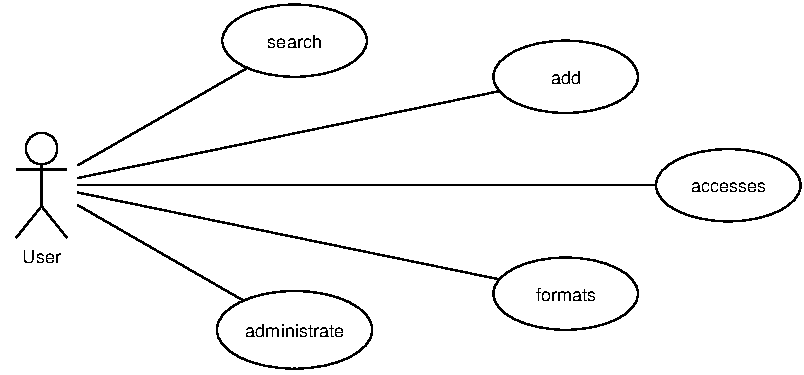
\includegraphics[width=.8\textwidth]{pics/ov-uc-001}
  \caption{Use case diagram (overview)}
  \label{fig:ov-usecase}
\end{figure}

\textit{Note:} Perhaps it is better to use the describe -- organise --
refer structure from \ref{sec:summrequ} supra?

\newenvironment{usecaselist}{%
\section{Usecases}
\label{sec:requsecase}
\tablehead{\firsthline}
{\tabletail{\lasthline}}
\begin{center}\begin{supertabular}{|l|p{11cm}|p{3cm}|}}
  {\end{supertabular}\end{center}}

\newcommand{\ucitem}[4]{#1& \textbf{#2} #3& #4\\}


% \begin{table}[htbp]
%   \centering
%   \begin{tabular}[t]{|l|p{.8\textwidth}|}
% \hline
% \textbf{\sffamily Use case} & \textbf{\sffamily Description}\\
% \hline

\begin{usecaselist}
\input{tx-use.lst}  
\end{usecaselist}





% \hline
%   \end{tabular}
%   \caption{Activities (use cases)}
%   \label{tab:ov-usecase}
% \end{table}

\newpage

\cbstart 


\section{Requirements Directory}
\label{sec:reqrequ}

The following table directs you to the detailed lists of functional
requirements that are distributed over this document. 

\begin{enumerate*}
\item Generalities
  \begin{enumerate*}
  \item Packageing and Installation
  \item Documentation
  \item Authorisation and Protection
  \end{enumerate*}
\item Bibliographical description
  \begin{enumerate*}
  \item Generalities
  \end{enumerate*}
\item Subject description and access 
  \begin{enumerate*}
  \item Generalities
  \item Persons
  \item Subject Headings 
  \item Classifications
  \item Coded lists and Classifiers
  \item Keywords, etc.
  \item Full text search
  \end{enumerate*}
\item User Interface, Input, and Import
  \begin{enumerate*}
  \item GUI generalities
  \item Manual Data Entry
  \item Editing and Checking
  \item Import facilities
  \item Spellchecking and Other Assitive Techniques
  \item Duplication Checking
  \item Accessibility and misc.
  \end{enumerate*}
\item Searching, Formatting, Display, and Output
  \begin{enumerate*}
  \item Generalities
  \end{enumerate*}
\item Annotations, Actions, Extensions
  \begin{enumerate*}
  \item Generalities
  \end{enumerate*}
\item API, Interfaces, Services
  \begin{enumerate*}
  \item Generalities
  \end{enumerate*}
\item Miscellaneous, dubious, ad interim
  \begin{enumerate*}
  \item Duplication checking
  \item Character sets
  \item Indexing
  \item Query service
  \end{enumerate*}
\end{enumerate*}


\cbend




\section{Objects and Classes -- the problem domain}
\label{sec:ov-domain}




\subsection{Interfaces}
\label{sec:ov-interface}


\section{Other Requirements}
\label{sec:reqother}



\section{Constraints}
\label{sec:reqconstr}



% IT-Sicherheitsziel
% Bedrohungs- und Risikoanalyse
%  IT-Sicherheit
% Fachliche Anforderungen


% 7. 1. Technische Randbedingungen


% 7. 2. Organisatorische Randbedingungen

% 7. 3. Sonstige Randbedingungen

% Randbedingungen, die weder technischer noch organisatorischer Natur
% sind, sind zu fixieren (z. B. 
% zeitliche und wirtschaftliche Randbedingungen).  

%%% Local Variables: 
%%% mode: latex
%%% TeX-master: "DG"
%%% End: 


\chapter{Architecture Overview}
\label{cha:archiview}

This chapter describes the architecture and components.


\section{Application Core}
\label{sec:archicore}

\Pyb\ provides access to \textbf{Databases} of bibiographical
informations and \textbf{Documents} (\textbf{Resources}). It allows
\textbf{Users} to store and retrieve records in an \textbf{internal
  Database}, including the ability to import the results of
\textbf{Queries} against external databases.  

It organises the stored records in \textbf{Lists} and
\textbf{Folders}, maintains \textbf{Indexes} on various attributes,
as well as \textbf{Authority files}, such as for \textbf{Persons},
\textbf{Subject headings}, \textbf{Classifications}, and other
\textbf{Descriptors}. 

Items in the database can be equipped with \textbf{Annotations}; these
include \textbf{Actions} that are requested (and assorted status),
\textbf{Abstracts} or \textbf{Notes} reflecting the contents, and also
\textbf{Quotations} taken from the source document, structured
\textbf{Case annotations} for further processing, and also
\textbf{Proxy references} to external documents which might serve the
same purposes. 

\textbf{Holdings} are recorded, which include references to electronic
copies as well as shelf numbers or other location information, both at
the user's site or any other institution, anywhere.

The bibliographical \textbf{Description} allows for
\textbf{Extensions} to deal with e.g., special materials.  For
multi-level description a \textbf{Hierarchy} of items is created. 

Items may be assigned a \textbf{Security Label}, to restrict their
dissemination. 

Items are formatted according to \textbf{Formats} that are user
selectable and -definable. 


\section{Architecure Baseline}
\label{sec:archibase}


\section{Implementation Plan}
\label{sec:archiplan}




%%% Local Variables: 
%%% mode: latex
%%% TeX-master: "DG"
%%% End: 

\part{Design Considerations}
\section{The Graphical User Interface}
\label{sec:gui}


In this chapter we discuss the user interface, in our case based on
the \textsf{Gtk\,2.0} toolkit. First we give an overview of the user
interface elements, then we look at the rewuirements of individual
widgets.

\textbf{See also:} For the integration of Pybliographer into Word
Processors and Browsers, see section \ref{sec:wpintegr}; for using
Pybliographer from the commandline or scripts, see chapter
\ref{sec:scripting}.



\subsection{Major elements of the user interface}
\label{sec:guimajor}


\ref{sec:docrequest}




\subsection{Displaying and Using Indices}
\label{sec:guiindex}


The usual way of perusing a bibliography or a catalogue is by means of
a listing, either according to the author's name, or according to the
title, a keyword, or any other suitable piece of information. 

With online catalogues, one usually has access to the underlying
(technical) \textit{indices}, if only to compensate for the
limitations of usual search facilities and the missing overview
possible with today's display devices. 

It is best to have multiple indices (Indexviews), so as to make best
use of the structure of the data (e.g., the \textit{Person or Author
  Index} would usually show the works of the author upon selection (as
a tree view) not the authority record of the author, a title index
might in a similar way allow subordinate entries for editions or
translations, etc. 

Sometimes special indices are required. A manuscript collection might
want to enter and find listed the first few words of a manuscript or
letter, a specialist might need the names of translators, or scribes,
or printers. So ther must be a degree of configurability in addition
to that needed to cater for the differing tastes and traditions.

\subsection{Accelerator Key Assignments}
\label{sec:keys}

Accelerator keys allow easy selection of functions, in particular easy
switching of views, which is in paricular desireable when doing data
entry and editing. These are activities which repeatedly and
predictably need a great number of screens to proceed, switching them
with the mouse is particularly unpleasant. 
Consitent assignment of \textit{shortcuts} is needed.



%%% Local Variables: 
%%% mode: latex
%%% TeX-master: "td-td1"
%%% End: 

\section{Organising and Manipulating References }
\label{sec:basicwork}

One aspect of Pybliographer is its use to \textit{organise references}
-- that lays the accent onto the varieties of uses that these
references could be put to, and the concomitant variety of possible
organisation we have to cope with. This de-emphasises the
bibliographical description, as a rule, but stresses our ability to
annotate and link.



As a rule, our data is kept in one database, organised into
\textit{folders} (compare Biblioscape \ref{biblioscapefolder}). 

A variety of \textit{Indices} are kept  to allow fast access. q


%%% Local Variables: 
%%% mode: latex
%%% TeX-master: "todo"
%%% End: 

% $Id$

\section{Searching, Selecting, and Formatting Data}
\label{sec:processing}


A \textit{search} is an operation that is performed against one or
more \textit{databases} -- usually locally represented by
Pybliographer and remotely by database servers known as
\textit{connections} -- and that results uniformly in a \textit{result
  set}.

As a rule, such a result set is if necessary \textit{imported} as such
into the Pybliographer database, and sooner or later \textit{selected}
from.

A \textit{selection} is any subset of the database, usually the result
of manually inspecting (\textit{scanning}) some result set, that is
presented to a processing option: either to be set apart for further
processing at a later time, or to be processed by the output routines
in order to be presented or exported.
[XXX Are there other uses? ]



\paragraph{Notes:}

\begin{itemize}
\item Results sets can vary considerably in size. Efficiant means of
  handling them are important.
\item Various situations are to be considered and equally suppported
  \begin{itemize}
  \item One looks up price/holdings/availability information for an
    already known title.  That should result in the new information
    being added to the existing entry (and perhaps the latter being a
    bit improved). Possible actions include posting a note to pick up
    the book at the next visit to the library, or to make a copy from a
    journal, or to order it from the bookseller or the ILL service.
  \item One browses several data bases and cumulates the
    results. Later one reduces the set and adds it to the data base.
  \item One adds, perhaps on a regular schedule, records from an
    external source. Evidently this situation calls for other
    mechanisms and tools than the previous one, in spite of its
    superficial similarity. 
  \item On builds a bibliography or similar documentation database --
    involves most of the above situations and adds requirements for
    stringent administrative control. 
  \end{itemize}
\end{itemize}



\subsection{A generic query service}
\label{sec:genquery}

The exact possibilities that a database provides for searching are as
manifold as are the data. Paradoxically this makes it more easy to
provide one integrated query service -- any attempt to equip every
database and every service with its own query interface cannot but
falter in view of the enormeous programming investment that would be
needed.

It's not clear, perhaps, how the individual services can communicate
their capabilities upwards towards the query service, but it should be
evident that \textit{some} communication would be helpful -- even if
one fully acknowledges that the assessment of a database service must
usually include information that is not available to the
program. (Example: cataloguing rules -- RAK, AACR, \dots)





\subsection{Integration with editors, wordprocessors, and browsers}
\label{sec:wpintegr}
\task{wpintegration}

Integration with editors like Emacs, word processors like Abiword, and
bowsers like Mozilla enhances ease of use, broadens its field of
application and reduces user's keystrokes and thus the opportunity for
errors on his side.

We distinguish the following use cases:
\begin{description}
\item[Adding a citation] When writing, the user wants to add a
  reference to certain document, of which he might remember no more
  than some words from the title, or the author, or even less, but
  as a rule, not the exact citation key that Bib\TeX\,e.g., would use
  to identify it.

  The user should refer to the document by selecting from a result set
  or shortlist. 
\item[Inserting citations] Quite often the case arises that a document
  must be cited in, say, an email without wanting the whole (Bib\TeX)
  machinery  to be put in action. 
  
  A simply formatted citation could be offered via \textit{Drag and
  Drop}.
\item[Annotating] When reading, the user wants to add a note. 
  
  He is helped with creating and maintaining annotations to documents
  (registering them with Pybliographer); annotations can be large and
  are not suitable for storage \textit{in} the bibliographical record,
  but a link could. On the other hand it is conceivable to point back
  from the annotation to the document, so it could stand on its own.
\item[Viewing documents] An electronic document could be requested.

  Define appropiate viewers and requestors (mainly for eprints -- the
  rest is more simple).
\item[Extracting metadata]  An electronic document is perused and the
  wish is that it be catalogued.
  
  A limited bibliographical description can be build from the metadata
  that is stored and communicated with the document.
  \textit{Importantly:} If downloaded, the local file address should
  be stored as well.
\end{description}
\subsubsection{Emacsen}


\subsubsection{Other editors}


\subsubsection{Mozilla}


\subsubsection{Other browsers}



\subsubsection{Kword}


\subsubsection{Abiword}


\subsubsection{Open Office}


\subsubsection{Other word processors}



\subsubsection{Other applications}



\subsection{Formatting references  and bibliographies}
\label{sec:formatting}


\subsection{Other applications}
\label{sec:applications}

[Connecting to OPACS, etc. ]

%%% Local Variables: 
%%% mode: latex
%%% TeX-master: "td-td1"
%%% End: 

% $Id$

\section{Interfacing to  External Ressources}
\label{sec:external}





\subsection{Connecting to external databases}
\label{sec:extconn}

Pybliographer uses \textit{connections} to external ressources for the
following purposes:
\begin{itemize}
\item To look up a catalogue (for immediate consumption, so to say),
  i.e., as a client program.
\item To obtain, as a result of a query, additional data for import.
\item To obtain additional documents that are referred to from the
  data base, i.e., via an \textit{URL} or an \textit{Eprints} link.
\item To perform operations on the remote system, i.e., to request
  books or copies by means of an \textit{OPAC}. 
\item \Think To cooperate with other Pybliographers, sharing and
  updating data.

\end{itemize}

% Query processing


% * Configuration

%   A list of available connections (databases) is built during start-up
%   (from pyblio.xml) Note that this precludes specialised parsing. 

%   It would be nice to have a configuration dialogue. 

% * Query dialogue

%   Presents a dropdown list of such servers (but allows local search as
%   well). 

%   Determines and loads extension module. (Using 'type' atttribute.)

%   Builds Query object.

% * Extension module

%   Reads and sets parameters (stored during start-up). 

%   Customises query:
%   - marks fields available for search
%   - add-on options for query dialogue (in preference to:)
%   - expert search dialogue

%   Builds request (object) -> Query.request.
  
% * Query requestor

%   Sends request and receives result.  Error processing.
   
%   Determines and loads Importer module. 
%   Builds an Import object. Feeds result data to import module.



\subsection{Writing Import Filters}
\label{sec:importfilter}

Import filters are used not only when a \textit{file} is imported, in
a narrow sense, but also when opening a file, and, perhaps more
importantly, when processing the results of a \textit{query}.

An \textit{Import Module} provides the needed support. Typically, there
is one such module for every major data format, say MARC or Bib\TeX.

A major part of such a module is a Reader class, which subclasses (is
derived from, and specialises) the class \texttt{ImportReader} in the
module \texttt{Pyblio.Import}. 

In fact, most Reader modules do not derive directly from
\texttt{InportReader}, but from an intermediary, as
\texttt{TaggedReader} for data structured as a sequence of tagged
fields, like in the MARC format, \texttt{TextReader} for data that
comes as `unstructured' text, like taken from the references of an
article, \texttt{XmlReader} for XML formatted text.

In this way, we have a \textit{framework} for import modules, one that
makes writing or modifying an import reader much more simple. This is
important, because requirements and interface continue to evolve. 

The format specific modules are not the end of the story, yet. For
one, a format like MARC is in fact so vast that it will probably never
be completely implemented and used, neither by a library, nor by
Pybliographer. It is, however, to be expected that one time or the
other, someone would be better off if he could make use of that exotic
feature, and would be happy to add support. In addition, one may
encounter a situation in which the standard processing is inadequate
and better be modified.  Thus it is useful to be able to have an easy
way of adapting to one's very special needs, be it in terms of adding
or of overriding standard behaviour, i.e., methods.

There is yet another point to be made. A framework is also a way of
sharing the implementation effort. That means that adding code to the
common base is more attractive  and this in turn makes the use of
Pybliographer more attractive. So  everone profits. 



\subsubsection{Framework Services}




The base and intermediate classes, the framework, provide the
following services and features: 
\begin{description}
\item[Input] The source data is accepted by various means: files,
  iterators, in-core objects, and made available in a standardised way
  to the processing. 
\item[User interfacing] The user interface, always requiring a big
  programming effort, is structured by the base classes (togerther, of
  course, with the Gui Component), thus sharing a lot of work.
\item[Data handling] In the past, the handling of the input data was
  almost completely left to the format specific code, resulting in an
  enormous duplication of code and often poor exploitation of the
  source data. With the new design, most of the semantic data handling
  will be done by functions in specialised modules, sharply
  distinguishing between the parsing (syntactic) and database aspects
  of the task.
\item[Duplication checking] Like the user interface, the duplication
  check is an example of a pragramming task, that is not easily
  undertaken within the confines of one particular application, but
  only if it can be done wholesale. 
\item[On- and offline correction] It is highly desirable to be able to
  correct imported data in a systematic way, the framework will provide
  for that, both during inital processing, dubbed on-line, as well as
  at a later time.
\item[Customisation] There are ways to adapt the import processing
  which can be done easily in a generic way.  It is, e.g., simple to
  exclude all data from certain categories (tags) from further
  processing and therefore \texttt{TaggedReader} provides a parameter
  to specify such tags -- it can even be done interactively from an
  options dialogue. No programming needed.
\item[Data management aspects] The data imported will be kept
  logically identified as long as it is desired, without the need to
  keep separate files for it. That remedies a major problem with the
  work organisation in the past and it is necessary in any way for a
  data base oriented Pybliographer.
\end{description}



\subsubsection{Class hierarchy}

The fundamental class is \texttt{ImportReader} in Module
\texttt{Import.py}. It implements an \texttt{Iterator} interface,
viz.\ \texttt{first()} and  \texttt{next()} methods. 

\begin{verbatim}
class ImportReader (Iterator.Iterator):

    """Base class for all import reader classes.

    Support for input methods, encodings, database and GUI connections, 
    """

### The following need no change as a rule:
    def first (self):
        return self.next()

    def next (self, entry=None, data=None):
        """Process the next entry from the input source.
        entry and data argument are provided for easy testing."""

        e = entry or self.next_entry()
        x = data or self.read_next()
        if self.options.has_key('preserve_input'):
            e.lines = x
        self.entry = e
        return self.parse(x)

\end{verbatim}

Subclasses will need to provide, among others, implementations of
\texttt{read\_next} and \texttt{parse}.

A typical implementation of \texttt{parse} from \texttt{TaggedReader}
follows: 
\begin{verbatim}
    def parse (x):

        self.begin_record(x)
       
## it may be convenient, if the read_next routine already assembles
## continuation lines. Let's assume this

        for i in x:
            tag = i[0:self.tagcol]
            data = i[tagcol:]

            if discardrx and discardrx.match(tag):
                continue
                      
            if _cache.has_key(tag):
                _cache[tag] (self, tag, data)
            else:
                methname = 'do_'+str(tag)

                if hasattr(self, methname):
                    method = getattr(self, methname)
                else :
                    method = self.do_tag
                    
                method(self, tag, data)
                _cache[tag] = method

        self.end_record(x)
        return self.entry

\end{verbatim}

So in this case, for a tag `XYZ', a subclass implemented method
`do\_XYZ (self, tag, data)' would be called, if it exists. If not,
`do\_tag' would be called and as a rule, distinguish according to the
tag, as directed by parameters of the class, whether to ignore, or to
store (in a generic way) the data. 


\subsubsection{Class parameters}


\paragraph{Control objects}

\begin{description}
\item[control=None] specifies the associated control object.
\end{description}


\paragraph{Input} Three possibilities are provided for. The data
parameter is particularly useful for testing. \textit{One and only one
must be selected from the following}

\begin{description}
\item[file=\textit{filename}] if input is from a file,
\item[data=\textit{data object}] if input is from an incore object,
\item[iter=\textit{iterator}] if an iterator is specified.
\end{description}


% * Import module

%   Parses result data. Builds result set -> Import.set

%   Special processing:

%   - On-/Off-line correction.
%   - Checking for duplicates.
%   - Checking against author, journals, etc. database.
%   - Flexible handling of input data (store it, ignore it, ...)
  
%   Marks (and displays) the import set as a whole for reference.

% * Control objects

%   Saved in configuration file.
  
%   Static: Connection
%   Dynamic: Query, Import 

  





\subsection{Writing Export Filters}
\label{sec:exportfilter}


\subsection{Pybliographer as Web Server }
\label{sec:pybweb}


\subsection{Requesting remote operations}
\label{sec:remotereq}


\subsection{Requesting documents}
\label{sec:docrequest}

Given an entry that refers an electronic document, it is an easy idea
to consider requesting it by mouse-click, so to say.



%%% Local Variables: 
%%% mode: latex
%%% TeX-master: "td-td1"
%%% End: 

% $Id$

\section{Bibliographic Data: types, formats, schemata}
\label{sec:bibdata}


\subsection{Bibliographical Objects}
\label{sec:bibobject}

See the IFLA report.

\subsection{Persons}
\label{sec:persons}



\subsection{Works}
\label{sec:worksasobj}


\subsection{Subjects}
\label{sec:subjectsasobj}





\subsection{Database Organisation}
\label{sec:database}






%%% Local Variables: 
%%% mode: latex
%%% TeX-master: "td-td1"
%%% End: 

% $Id$

\section{Scripting and Configuration}
\label{sec:scripting}

%%% Local Variables: 
%%% mode: latex
%%% TeX-master: "td-td1"
%%% End: 

%$Id$
\newenvironment*{TodoItem}[6][]{%
\begingroup\noindent\textbf{\textsf{#2\quad #6}}\leftskip10pt\\}
{\endgroup}
\section{Technical Questions}
\label{sec:techne}


\subsection{Architectural issues}
\label{sec:tec-archi}


\subsection{Compatability issues}
\label{sec:tec-compat}

\begin{TodoItem}{0016}{}{}{}{Remain compatible with BibTeX}
\end{TodoItem}


\subsection{Charset and markup issues}
\label{sec:tec-chars}

\begin{TodoItem}{0001}{}{}{}{Establish Unicode internally and for
    storage}
\end{TodoItem}

%%% Local Variables: 
%%% mode: latex
%%% TeX-master: "td-td1"
%%% End: 

\part{Component Design}

\include{td-ker}

\include{td-coc}

\include{td-sto}

\chapter{The Bibliographic Component}
\label{cha:bibco}

\begin{description}
\item[Purpose] Description of resources; with accent upon the
  classical bibliographical data (types). -- Contains the core of the
  application domain objects.
\item[Modules] Biblio\dots
\item[External Dependencies] Depends on GUI for display interaction
\item[Internal Dependencies] Depends on Storage for persistence, on
  Common Control for a little configuration and interaction support,
  on Writer for formatting.
\item[Initialisation] Primary DB provides needed configuration and
  control data. Some bootstrapping and fallback mechanism desirable.
\end{description}



\section{Description}
\label{sec:bibcodesc}

\begin{dnote}
  \item It is to be determined, how much of the application domain is
  to be catered for by this package-component. 
\item Demarkation against Storage and Writer seems clear to me, 
\item Candidates for related packages are IMHO Topics, Annotations,
  Holdings 
\end{dnote}

The bibliographical description lies at the heart of \Pyb, together
with the features for annotation and organising of references.

This package provides:
\begin{itemize*}
\item description up to recent ISBD developments, including
  multi-level description and material specific description
\item extensible efficient indexing
\item customisable, assisted  data entry (spellchecking)
\item extensible structured description (case analysis)
\item annotation, integration of external documents w.r.t. searching
\item task-oriented (writing) support 
\item maintenance of associations between bibliographical objects
\item maintenance of classifications, etc.; effient use thereof
\item (some of the above should be expanded upon, in particular the
  following question should be answered: what is the specific
  \textit{bibliographical} content, and what is just generic?
  Example: versions of a document, translations, reviews: how are the
  related?)
\item extensions for collections, archival resources
\end{itemize*}

%%% Local Variables: 
%%% mode: latex
%%% TeX-master: "DG"
%%% End: 

\cleardoublepage
\appendix
\part{Appendices}

%% $Id$

\section{Programming Tasks}
\label{sec:app:tasks}

Some other things to do XXXX
\begin{itemize}
\item Sort order according to German standards
\item Handling German \textit{Umlaute} -- � � � -- 

\end{itemize}

%%% Local Variables: 
%%% mode: latex
%%% TeX-master: "todo"
%%% End: 



% $Id$

\section{Features of commercial products}
\label{sec:commfeat}

\subsection{Biblioscape}
\label{sec:biblioscapefeat}


                                                               
%\textbf{Biblioscape 4 Feature Matrix}


\textit{Organize references with folders, dynamic folders, etc.}
\begin{itemize}
 \item[Folder] \label{biblioscapefolder}
Add references into folders. One reference can be put into
 multiple folders without creating a duplicate. Organize references
 into folders with drag and drop.

 
 \item[Dynamic folder] Organize and save queries into a tree structure.
 All references meeting the search criteria will be listed under a
 dynamic folder.

 \item[Indexed search] Return search results in a couple of seconds no
 matter how big the database is. One line search works the same
 way as most Internet search engines. Supports logical searches,
 fuzzy searches, etc.

 \item[Import filter] Bibliographic data from any data sources can be
 imported with a proper import filter. User can create new or edit
 existing import filters.

 \item[Output style] References can be displayed any any style like MLA,
 APA, etc. A large number of styles are provided for different
 journals. Users can also create new ones.

 \item[Cross linking] Link a reference to other references in the same
 database. You can define a relationship for the links, like
 "Supportive", "Contradict". You can also add comments for each
 link.

 \item[Navigation view] A reference can be displayed in an organizational
 chart where each node can lead to related records.

 \item[Formatted preview] Display a reference as formatted text
 according to the active output style. 

 \item[Live preview] Display data fields of the selected reference in a grid
 without opening it. Changes made to the data will be saved to
 database as you move to another record.

 \item[Graphics and OLE] If a reference has associated graphics and OLE
 objects, add them to the Document field. The document field can
 be used to store the full text of a reference.

 \item[Field lookup] List all unique values along with the number of
 occurrences of a data field. All data fields with possible repeated
 values can be shown in lookup view. These include Author,
 Keyword, Publisher, Language, Country, Subject, etc.

 \item[Recycle bin] All deleted references are put into the Recycle bin.
 You can recover them from the Recycle bin or remove them
 permanently from the Recycle bin.

 \item[Advanced search] Query any data field with a visual query builder.

 \item[Find and Replace] Search for a word or phrase and limit the search
 to a data field or all data. The same is true for the Replace
 operation.

 \item[Sorting] Sort a column by clicking on the header. Click again and
 the column will sort in reverse order. User can also define
 multi-level sorting.

 \item[Filtering] Define a filtering criteria with a visual filter builder and
 apply the filter to any dataset.

 \item[Term list] Users can keep frequently used phrases in a term list.
 Terms can be organized in the list by category.

 \item[Move field] The content of a data field can be moved from one
 field to another.

 \item[Global edit] The content of a data field can be changed at once
 for all selected references.

 \item[Eliminate duplicates] Duplicate records can be found and
 removed. Fuzzy search is supported for finding duplicates.

 \item[Analyze references] Data fields in the reference table can be
 analyzed for data distribution.

 \item[SQL commands] Users who are familiar with SQL can query the
 database directly with SQL commands.

 \item[Report] A built-in database report writer will a print data report,
 including a subject bibliography grouped by keyword, author, year,
 subject, etc.

\end{itemize}
\textit{Format papers to generate citations and bibliography}

\begin{itemize}
\item  [Format a paper] Convert the temporary citations of a document
 into formatted citations and a bibliography.

 \item[Unformat a paper] Convert a Biblioscape formatted paper back to
 unformatted form (with temporary citations) so citations can be
 added or deleted before the final formatting.

 \item[Word support] Full integration with Microsoft Word, Biblioscape
 menus and toolbar can be added to the Word menu and toolbar
 system.

 \item[WordPerfect support] Full integration with Corel WordPerfect,
 Biblioscape menus and toolbar can be added to the WordPerfect
 menu and toolbar system.

 \item[Other word processors] Biblioscape methods for word processors
 integration are published and open to all word processors that
 support DDE.

 \item[HTML support] Biblioscape can generate formatted papers in HTML
 format. A hyperlink can be created automatically between an
 in-text citation and its reference in a bibliography.

 \item[Natural citation] Use words or phrases to uniquely identify a
 reference in a temporary citation instead of using a Reference ID.
 If references are moved into another database, temporary citations
 don't need to be changed.

 \item[Cite while you write] Use BiblioSidekick to display references in a
  small, always on top windows. While in a word processor like Word
 or WordPerfect, just drag and drop the selected reference in the
 place where you want to cite it.

 \item[BiblioWord] A full featured word processor inside Biblioscape. Just
 drag selected references from a panel on the right when you want
 to cite. BiblioWord supports live spelling check, thesaurus, tables,
 graphics, OLE, multi-level undo, etc.

\end{itemize}

\textit{Access the Internet to capture bibliographic data, Web pages}
\begin{itemize}

 \item[Remote databases] Access thousands of remote bibliographic
 databases on the Web with an integrated Web browser. These
 sites include university sites, commercial databases, and
 government sites. Most of them are free.

 \item[Capture references] Search web based bibliographic databases
 from inside Biblioscape, click a button to capture search results
 into a Biblioscape database with the right import filter. New import
 filters can be created by users.

 \item[Capture Web pages] Research on the Web with the Biblioscape
 integrated browser, capture a web page into a Biblioscape
 References table or Notes table. All words in the Web page will be
 indexed for future search. Graphics and links are captured along
 with the page.

 \item[Resources] A directory of bibliographic resources on the Web. Each
 entry listed has an associated import filter. The local Resources list
 can be expanded and edited by the user.

 \item[Web directory] Biblioscape Web site lists a collection of sites
 valuable to researchers. Web sites are organized by subject.
 Bibliographic databases are the main part of the listing. Although
 other types of Web resources are also listed.

 \item[Z39.50] Most Z39.50 enabled bibliographic databases also have a
 Web interface, Biblioscape's integrated Web browser can be used
 to search such sites and capture search results directly into a
 database. 

 \item[Link to a note] Easily create a link between a note and a Web site.

\end{itemize}


\textit{Take notes and link them to references, tasks, web sites, etc.}

\begin{itemize}
 \item[Tree structure] Organize notes in a tree structure. Note's position
 in the tree can be rearranged by drag and drop.

 \item[Indexed search] Find your note fast with indexed search. Each
 word in your Notes database is indexed for super fast search. The
 search words are colored in red on the hit page. Indexed search
 supports logical operators, wildcards, fuzzy search, etc.

 \item[Advanced search] Limit your search to a data field like Date
 Created, Keywords, etc. Build complex searches with a visual query
 builder.

 \item[Format text] The text in your note can be formatted with all the
 standard options, including fonts, color, background color,
 superscript, subscript, paragraph alignment, bullet list, number list,
 etc.

 \item[Link] Each note can be linked to other notes, references, tasks,
 catalog items, Web URLs, local files, etc. Double clicking on a link
 will take you to the linked item.

 \item[Web capture] Notes can be used to organize captured Web pages.
  All the graphics and hyperlinks of captured web pages can be
 properly displayed.

 \item[Table support] You can insert tables in your notes. Additional rows
 can be added and deleted.

 \item[Find and Replace] Standard Find and Replace tools for finding and
 replacing text in your notes.

 \item[Graphics and OLE] Graphics can be added to your notes. OLE is
 also supported. Therefore, you can add chemical structure
 drawings, spreadsheets, CAD drawings, etc. in your notes.

 \item[Table view] The notes can also be displayed in a table besides the
 default tree view. Notes can be sorted and grouped in a table.

 \item[Keyword lookup] Each note can have associated keywords. These
 keywords can be displayed in a lookup list along with its number of
 occurrences. Double clicking on a keyword will retrieve all related
 notes.

 \item[Spelling and thesaurus] A powerful spelling checker is included.
 Additional dictionaries can be downloaded for all major European
 languages. A thesaurus is also included to help the user to find the
 right words during writing.

 \item[Icons] Each note can be assigned a different icon to distinguish it
 from other notes.

 \item[Export] Each note can be exported to a file in RTF or HTML format.

\end{itemize}

\textit{Manage tasks and organize your research ToDo list}
\begin{itemize}

 \item[Sort tasks:]Click on the column header to sort tasks, click again to
 sort in reverse order.

\item[Group tasks] Group tasks by Priority, Status, Date Created, etc.
]
 \item[Task progress] Track the progress of a task by marking its
 percentage completed.

 \item[Task creation] Create tasks inside References module, and add
 selected references into the Description field of the new task.

 \item[Link to a note] Create a link between a selected task and a note.

 \item[Advanced search] Search tasks with a visual query builder.

\end{itemize}

\textit{Draw a chart to present your ideas}
\begin{itemize}

 \item[Flow chart] Draw a flow chart with an easy to use chart editor.

 \item[Knowledge map] Draw a chart and link a chart object to other
 modules. For example, double clicking on a chart object will open a
 group of references, tasks, notes, etc. A SQL query can be
 associated with each chart object. A knowledge map can be built
 with such associated queries.

 \item[Tree structure] Organize your charts in a tree structure. The
 position of each chart in the tree can be rearranged by drag and
 drop.

 \item[Link to a note] Create a link between a chart and a note.

 \item[Zoom Display] options like zoom in and zoom out, actual size, and
 fit to screen are supported.

 \item[Icon] Each chart can have an icon associated and displayed.

 \item[Shape and color] The shape and color of each chart object can be
 customized. The label text can be displayed in different fonts and
 colors.

 \item[Connectors] Chart objects can be connected with a flexible
 connector which can be curved. A connector can have its own
 label, font, color, size, different sources and destination arrows,
 and link points.
 
\end{itemize}


\textit{Manage a library without a steep learning curve}
\begin{itemize}
 \item[Catalog] Manage library collection data into 56 data fields,
 organized into several groups including Bibliographic, Holding,
 Request, Order, Serial, and General.

 \item[Serials] Manage serials and related activities including tracking,
 routing, etc. 

 \item[Circulation history] Search, sort, and group circulation data.
 Display circulation activities by borrower, status, subject, etc. 

 \item[Check Out] Check out books for library patrons, add notes, easily
 change due dates.

 \item[Check In] Check in books returned by borrowers. Automatically
 reminds librarian about Hold status.

 \item[Renew] Renew books for borrowers, add a note. Find renewed
 items by ID or title.

 \item[Hold] Put a hold on a checked out book. Show a reminder when
 that book is returned.

 \item[Interlibrary Loan] Manage interlibrary loan requests, track loan
 status, log shippings, etc.

 \item[Borrowers] Manage borrower's information (address, phone, fax,
 email, et]c.)

 \item[Lenders] Manage lender's information (contact's name, phone, fax,
 email, notes, etc.)

 \item[Suppliers] Manage supplier's information (address, phone, fax,
 email, notes, etc.)

 \item[Sort] Click on any column header to sort then click again to sort in
 reverse order.

 \item[Group] Group data by drag and drop. Data can be grouped at
 multi-levels by any data field.

 \item[Field chooser] Choose which data fields to include in the data grid
 by drag and drop.

 \item[Report and print] Build or customize data reports with a powerful
 report builder. Users can create new reports with a wizard. New
 reports can be easily added to the menu system. Reports can be
 previewed, printed, or saved as a files.


\end{itemize}

\textit{Web enable your bibliographic database with one click}

\begin{itemize}

 \item[Web publishing] Publish databases on the Web with BiblioWeb
 server. No other web server required. Runs on any Windows 95, 98,
 Me, NT4, 2000 machine.

 \item[Indexed search] Search references with a powerful search engine.
 Enter search commands like you do with a Web search engine.
 Supports search keywords AND, NOT, OR, LIKE, NEAR, Wildcards,
 etc.

 \item[Advanced search] Limit searches to certain fields. Build complex
 queries with up to 3 conditions.

 \item[Add references] Users with a Write account can add new
 references to the database using a web browser.

 \item[Edit and delete] Users can edit or delete their own references over
 the web.

 \item[Import] Import references over the Web with the right import filter,
 so you don't need to enter references one by one.

 \item[Hyperlinks] Search results are displayed with hyperlinks. Clicking
 on the hyperlink will trigger a new search for related items.

 \item[Style] Marked references can be displayed in any of the output
 styles that exist in Biblioscape.

 \item[Export] Marked references can be exported in several formats to be
 easily imported into other programs.

 \item[Format papers] Users can even format a paper over the Internet.
 Temporary citations in a document will be converted to formatted
 citations and bibliographies.

 \item[User forum] Includes a user forum application, so you can host a
 web based forum without extra cost.


\end{itemize}

%%% Local Variables: 
%%% mode: latex
%%% TeX-master: "todo"
%%% End: 




\nocite{*}

\raggedright


\bibliography{pyblio}


\end{document}
